% \begin{figure*}[t] 
%     % \setlength{\abovecaptionskip}{-0.cm}
%     % \setlength{\belowcaptionskip}{-0.5cm}
%     \centering 
%     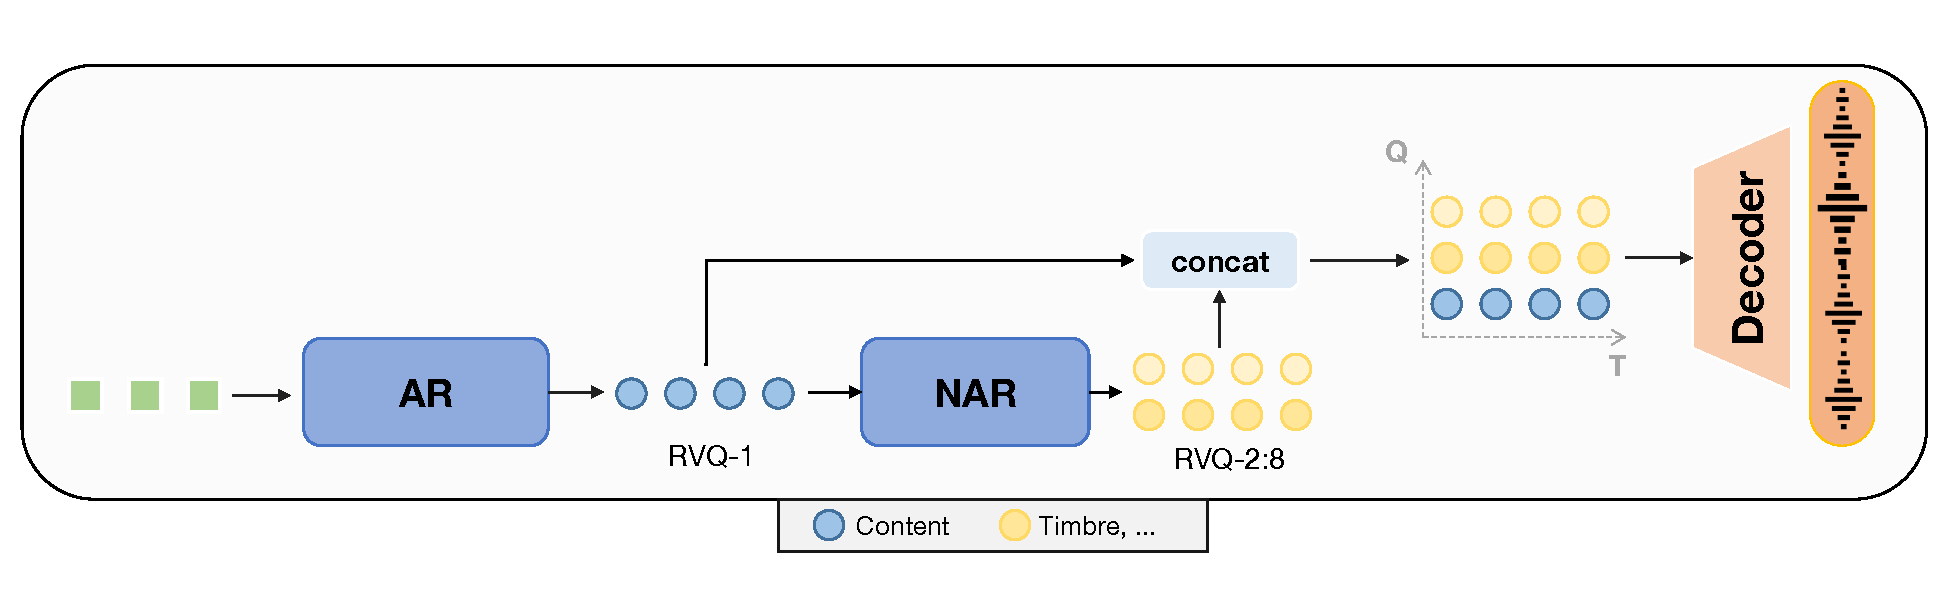
\includegraphics[width=1\textwidth]{Figures/ar_nar.pdf} 
%     \caption{Illustration of unified speech language models. AR refers to autoregressive and NAR refers to non-autoregressive. Speech
%     tokens are represented as colored circles and different colors represent different information.}
%     \label{fig:zs_tts} 
% \end{figure*}


% As shown in Figure~\ref{fig:zs_tts},
As shown in Figure~\ref{fig:token_model}, we can build a unified speech language model upon \method. Consisting of autoregressive and non-autoregressive models, it can hierarchically model information in speech. The autoregressive~(AR) model captures the content information by modeling tokens from the first RVQ quantizer. The non-autoregressive~(NAR) model complements paralinguistic information for the AR model by generating tokens from the subsequent quantizers conditioned on the first-layer tokens. 
We validate the effectiveness of unified speech language model on zero-shot TTS task. 
% USLM is available on \url{https://github.com/0nutation/USLM}.
% by comparing with VALL-E based on EnCodec. We keep model architectures, training and inference methods the same as VALL-E.

% AR model maps we train on the discrete tokens from the first quantizer $c^1$. It is conditioned on the phoneme sequence $i$ and formulated as
The AR model is built upon the first-layer tokens $\mathbf{c}_1$. Utilizing a transformer decoder-only architecture $\theta_{AR}$, we approach this conversion as a casual language modeling task with the phoneme sequence $u$ serving as the prompt for the AR model. The training objective can be formulated as
\begin{align*}
\mathcal{L}_{AR}=-\log\prod_{t=0}^{T}p(\mathbf{c}_1^t|\mathbf{c}_{1}^{<t},\mathbf{u};\theta_{AR}).
% p(c^{1}|i;\theta_{AR})=\prod_{t=0}^{T}p(c^{1}_{t}|c^{1}_{<t},i;\theta_{AR})
\end{align*}

% For NAR model, we train on discrete tokens from the second to the last quantizers $c^{2:8}$. It is conditioned on the first layer tokens $c^1$ and formulated as
The NAR model produces tokens $\mathbf{c}_{2:8}$ from the subsequent quantizers. Its architecture resembles that of the AR model, comprising eight distinct acoustic embedding layers and output prediction layers. To control the characteristics of the speaker’s voice, n acoustic prompt $\mathbf{\hat{C}}$ is employed for timbre guidance. The model is conditioned on phoneme sequence $u$, acoustic prompts $\mathbf{\hat{C}}$ and tokens from previous quantizers, leading to the formulation of the training objective as follows
\begin{align*}
\mathcal{L}_{NAR}=-\log\prod_{i=2}^{8}p(\mathbf{c}_{i}|\mathbf{c}_{<i},\mathbf{\hat{C}},\mathbf{u};\theta_{NAR}).
% p(c^{2:8}|i;\theta_{NAR})=\prod_{j=2}^{8}p(c^{j}|c^{<j},\mathbf{\hat{C}},i;\theta_{NAR})
\end{align*}


During inference, we convert text input to phoneme sequence and speech prompt to speech tokens. They are concatenated to form the prompts for AR and NAR models. Conditioned on that, the AR model generates first-level tokens, while the NAR model iteratively produces tokens of subsequent levels. The tokens generated by the AR and NAR models are then concatenated to construct the speech token matrix. Finally, we use the \method decoder to generate the waveform conditioned on the complete token matrix. 
